\lhead{\begin{tikzpicture}[remember picture, overlay]
     \node [anchor=100,inner sep=0] (imagenIZQUIERDA) at (current page header area.north){
\includegraphics[width=18cm]{18/img/Encabezado.PNG}};
     \end{tikzpicture}}
     \rhead{Angeles Hurtado}
     \rfoot{\begin{tikzpicture}[remember picture, overlay]
     \node [anchor=140,inner sep=0] (imagenDERECHA) at (current page footer area.south){
\includegraphics[width=18cm]{18/img/Foot.PNG}};
     \end{tikzpicture}}
     
     %----------------------------------------------------------------------------------------
     \lfoot{ \thepage}
     % \renewcommand{\labelenumi}{\alph{enumi}.)} 
     %----------------------------------------------------------------------------------------
     %----------------------------------------------------------------------------------------
     %	TITLE SECTION
     %----------------------------------------------------------------------------------------
     
     \setlength{\droptitle}{-5\baselineskip} % Move the title up
     \title{\textbf{Estudio de tiempos y movimientos en el ensamble de un circuito electrónico utilizando manuales con instrucciones}} % Article title
     
      \author{ 
      \textsc{Morales Piña  Cristian Jonathan}\\ 
     %  Afiliación:
      \texttt{ Instituto Tecnológico de Querétaro} \\ 
      \texttt{Tecnológico Nacional de México  } \\ 
      \texttt{Querétaro, MX}\\ 
      \texttt{lc22140573@queretaro.tecnm.mx)} 
      \and 
      \textsc{Ángeles Hurtado, Luis Alberto}\\ 
     %  Afiliación:
      \texttt{ Instituto Tecnológico de Querétaro } \\ 
      \texttt{Tecnológico Nacional de México } \\ 
      \texttt{Querétaro, MX}\\ 
      \texttt{.} 
     }
     
     
     %----------------------------------------------------------------------------------------
     
     % \begin{document}
     
     % Print the title
     \maketitle
     \thispagestyle{fancy}
     
     %----------------------------------------------------------------------------------------
     %	ARTICLE CONTENTS
     %----------------------------------------------------------------------------------------
     
     % \section*{Resumen}
     % \textit{Palabras clave:}
     % El resumen (ancho de página) deberá contener entre 100 y 200 palabras tipo Adobe Devangari 11 puntos.
     
     
     % 
     % 
     \textbf{\textit{Palabras clave}}: {Tiempos, ciclos, circuitos, movimientos e instrucción.}
     % \keywords{First keyword should be the corresponding to the research area according with the authors guide. Maximum of 6 keywords.}
     
     \section{Introducción}
     
     El estudio de tiempos y movimientos es una disciplina fundamental en la gestión de operaciones y la ingeniería industrial que se enfoca en analizar, medir y mejorar la eficiencia de los procesos de producción y trabajo. Este campo de estudio se remonta a los principios del siglo XX, cuando Frederick Winslow Taylor introdujo el concepto de "administración científica" para optimizar la productividad en las fábricas.
     
     El objetivo principal del estudio de tiempos y movimientos es identificar y eliminar desperdicios, reducir tiempos de ciclo, y mejorar la ergonomía y seguridad en el lugar de trabajo. Para lograr esto, se utilizan técnicas como la observación directa, la cronometría, el análisis de flujo de trabajo y la simplificación de tareas.
     
     Este estudio no solo se aplica en entornos industriales, sino también en sectores de servicios, salud y logística, donde la eficiencia y la optimización de procesos son cruciales para el éxito organizacional. En resumen, el estudio de tiempos y movimientos es una herramienta fundamental para impulsar la productividad, la calidad y la rentabilidad en cualquier tipo de organización.
     \textbf{La extensión máxima del artículo es de 8 páginas incluyendo figuras y referencias}. Los trabajos deberán ser de autoría propia y en caso de incluir material de terceros deberá señalarse apropiadamente en el área de “Referencias”.
     
     \section{Justificación}
     
     el ensamble de circuitos electrónicos es crucial debido a varios factores clave que afectan tanto la eficiencia operativa como la calidad del producto final. A continuación se presentan algunas razones que respaldan la necesidad de llevar a cabo este estudio utilizando diferentes métodos para su optimización
     
     \subsection{Optimización}
     
     La optimización es el proceso de encontrar la mejor solución posible para un problema específico dentro de un conjunto dado de restricciones o condiciones. En diversas áreas, desde las matemáticas y la ingeniería hasta la informática y la gestión empresarial, la optimización se utiliza para mejorar la eficiencia, minimizar costos, maximizar beneficios o lograr cualquier otro objetivo deseado. 
     La optimización puede realizarse utilizando una variedad de técnicas y herramientas, como algoritmos de optimización, análisis matemático, simulaciones y métodos heurísticos, entre otros. En última instancia, el objetivo de la optimización es encontrar la solución más eficiente y efectiva para un problema resuelto, teniendo en cuenta todas las restricciones y objetivos relevantes.
     
     \subsection{Descripción del problema}
     
     La principal problemática del estudio de tiempos y movimientos en el ensamble de circuitos electrónicos abarca una serie de desafíos que afectan la eficiencia, la calidad, la seguridad laboral y la rentabilidad del proceso. La aplicación de diferentes métodos de optimización es fundamental para abordar estos desafíos de manera efectiva y promover la excelencia en la producción de circuitos electrónicos
     
     \subsection{Fundamentación teórica}
     
     Estudio de métodos en el registro y examen crıtico
     sistemático de los modos de realizar actividades, con el
     fin de efectuar mejoras”. Se examinaran de los método para realizar actividades con el fin de mejorar la utilización eficaz de los recursos y establecer normas de rendimiento con respecto a las actividades. El objetivo es
     evaluar la forma en que se esta llevando a cabo el traba-
     jo con el fin de facilitar o modificar el enfoque con el que
     esta trabajando para reducir el tiempo y los movimientos
     innecesarios. Esto se realizara en base a los principios de
     la ingenierıa industrial los cuales proporcionan la base
     para entender como se pueden mejorar los procesos.
     
     Además de mejorar la eficiencia, el estudio de tiempos y movimientos también contribuye a mejorar la seguridad y la ergonomía en el lugar de trabajo. Al analizar y diseñar los movimientos de los trabajadores de manera cuidadosa, se pueden reducir los riesgos de lesiones y mejorar la calidad de vida laboral. \cite{niebel1980ingenieria}
     
     
     
     \section{Hipótesis}
     
     La aplicación de técnicas de análisis de tiempos y movimientos, junto con métodos de optimización, permitirá reducir significativamente los tiempos de ciclo en el ensamble de circuitos electrónicos, mejorando así la eficiencia del proceso.
     
     Se plantea que al optimizar los movimientos y métodos de ensamble, se reducirán los errores y defectos en el producto final, lo que resultará en una mejora general en la calidad de los circuitos electrónicos ensamblados.
     Se plantea que al analizar y optimizar los movimientos realizados por los trabajadores durante el ensamble de circuitos electrónicos, se mejorará la ergonomía de las estaciones de trabajo, reduciendo la fatiga y el riesgo de lesiones laborales.
     
     \subsection{Objetivo}
     
     El objetivo principal del estudio de tiempos y movimientos es mejorar la eficiencia en los procesos de producción y trabajo. Para lograr este objetivo, se persiguen varios objetivos específicos: 1. **Identificar ineficiencias:** El estudio de tiempos y movimientos busca identificar y eliminar cualquier actividad o proceso que no agregue valor al producto o servicio final. Esto puede incluir movimientos innecesarios, tiempos de espera o cualquier otro tipo de desperdicio.
     
     \subsection{Objetivos específicos}
     
     Reducir los tiempos de ciclo: Mediante la identificación y eliminación de actividades innecesarias, así como la optimización de los movimientos y métodos de ensamble, se busca reducir el tiempo total requerido para ensamblar un circuito electrónico, aumentando así la productividad y la capacidad de respuesta del proceso.
     
     Mejorar la calidad del producto: Al optimizar los tiempos y movimientos, se busca reducir la probabilidad de errores y defectos en el producto final. Esto se logra mediante la estandarización de procedimientos, la mejora de la precisión en el ensamble y la implementación de controles de calidad efectivos.
     
      Optimizar el uso de recursos: Se pretende utilizar de manera más eficiente los recursos disponibles, como el tiempo de trabajo, el espacio de trabajo, los equipos y los materiales. Esto implica minimizar el desperdicio y maximizar la utilización de los recursos para reducir los costos de producción y aumentar la rentabilidad.
     
      Promover la mejora continua: El estudio de tiempos y movimientos proporciona una base sólida para la identificación de oportunidades de mejora y la implementación de cambios efectivos en el proceso de ensamble de circuitos electrónicos. Se busca fomentar una cultura de mejora continua, donde se busque constantemente optimizar el proceso y adaptarse a los cambios en el entorno operativo. 
     
     \section{Cuerpo (Metodología, modelo matemático, etc.)}
     
     Se realizará el ensamble siguiendo el Manual de ensamble circuito electrónico ESP32-C6 para poder calcular la media y varianza desconocida, buscando generar datos históricos. 
         
          Una vez se obtengan los datos históricos se hará el análisis del ensamble por medio del MTM, que es una herramienta para la elaboración de entandares que da la posibilidad de evaluar una actividad u operación y a la vez los micro movimientos, los cuales tienen un valor en TMU (unidad de tiempo en MTM), para después ser representado en segundos, minutos y horas, por lo tanto permiten obtener un valor del tiempo de la actividad realizada por un operario.
          \cite{navarro2006estandarizacion}
          
          A continuación se muestra la lista de los materiales, la cantidad y el nombre de los mismos que son necesarios para el ensamble.
          Y a continuación de esta lista se muestra el Manual de ensamble circuito electrónico ESP32-C6.
     \section{Resultados}
     
     
     \section{Conclusiones}
     
     El operador puede realizar el ensamble sin ningún problema, siguiendo cada una de las instrucciones escritas o vistas en el manual, tomando un tiempo especifico y armando el circuito electrónica de forma ordenada y metódica. 
     \section{Agradecimientos}
     
     Al profe por ayudarme en Visual y a Blanck Diamont 
     
     \bibliographystyle{ieeetr}
     \bibliography{18/referencias}
      % 
     %   
     %%%%%%%%%%%%%%%%%%%%%%%%%%%%%%%%%%
     \appendix
     %%%%%%%%%%%%%%%%%%%%%%%%%%%%%%%%%%
     % 
     % 
     %%%%%%%%%%%%%%%%%%%%%%%%%%%%%%%%%%%%%%%%
     \centering{\section[\appendixautorefname{}]{Apéndice}}\label{anexo:materialesDeEnsamble}
     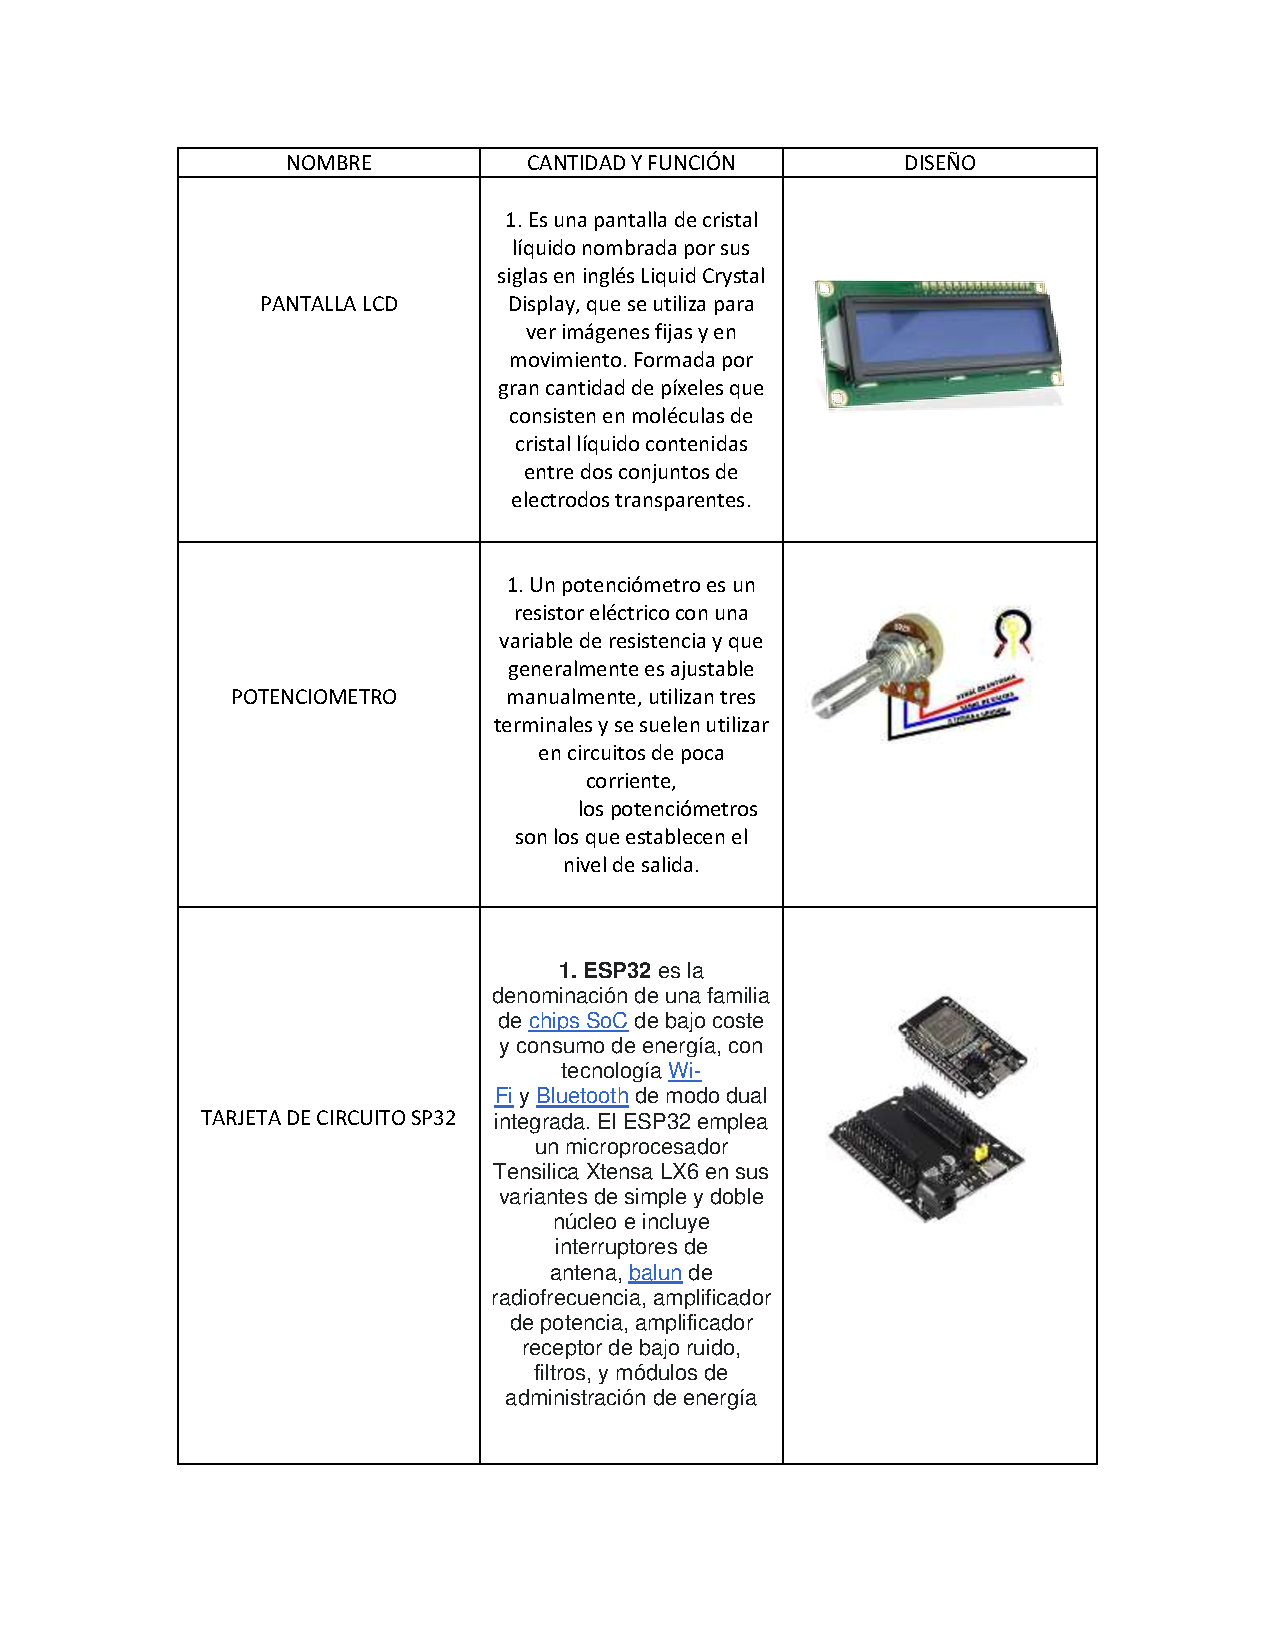
\includepdf[pages=-]{18/img/materialesDeEnsamble.pdf}
     %%%%%%%%%%%%%%%%%%%%%%%%%%%%%%%%%%%%%%%%
     %%%%%%%%%%%%%%%%%%%%%%%%%%%%%%%%%%%%%%%%
     \centering{\section[\appendixautorefname{}]{Apéndice}}\label{anexo:manualDeEnsamble}
     \includepdf[pages=-]{18/img/manualDeEnsamble.pdf}
     %%%%%%%%%%%%%%%%%%%%%%%%%%%%%%%%%%%%%%%%
     \centering{\section[\appendixautorefname{}]{Apéndice}}\label{anexo:resultadosDeEnsamble}
     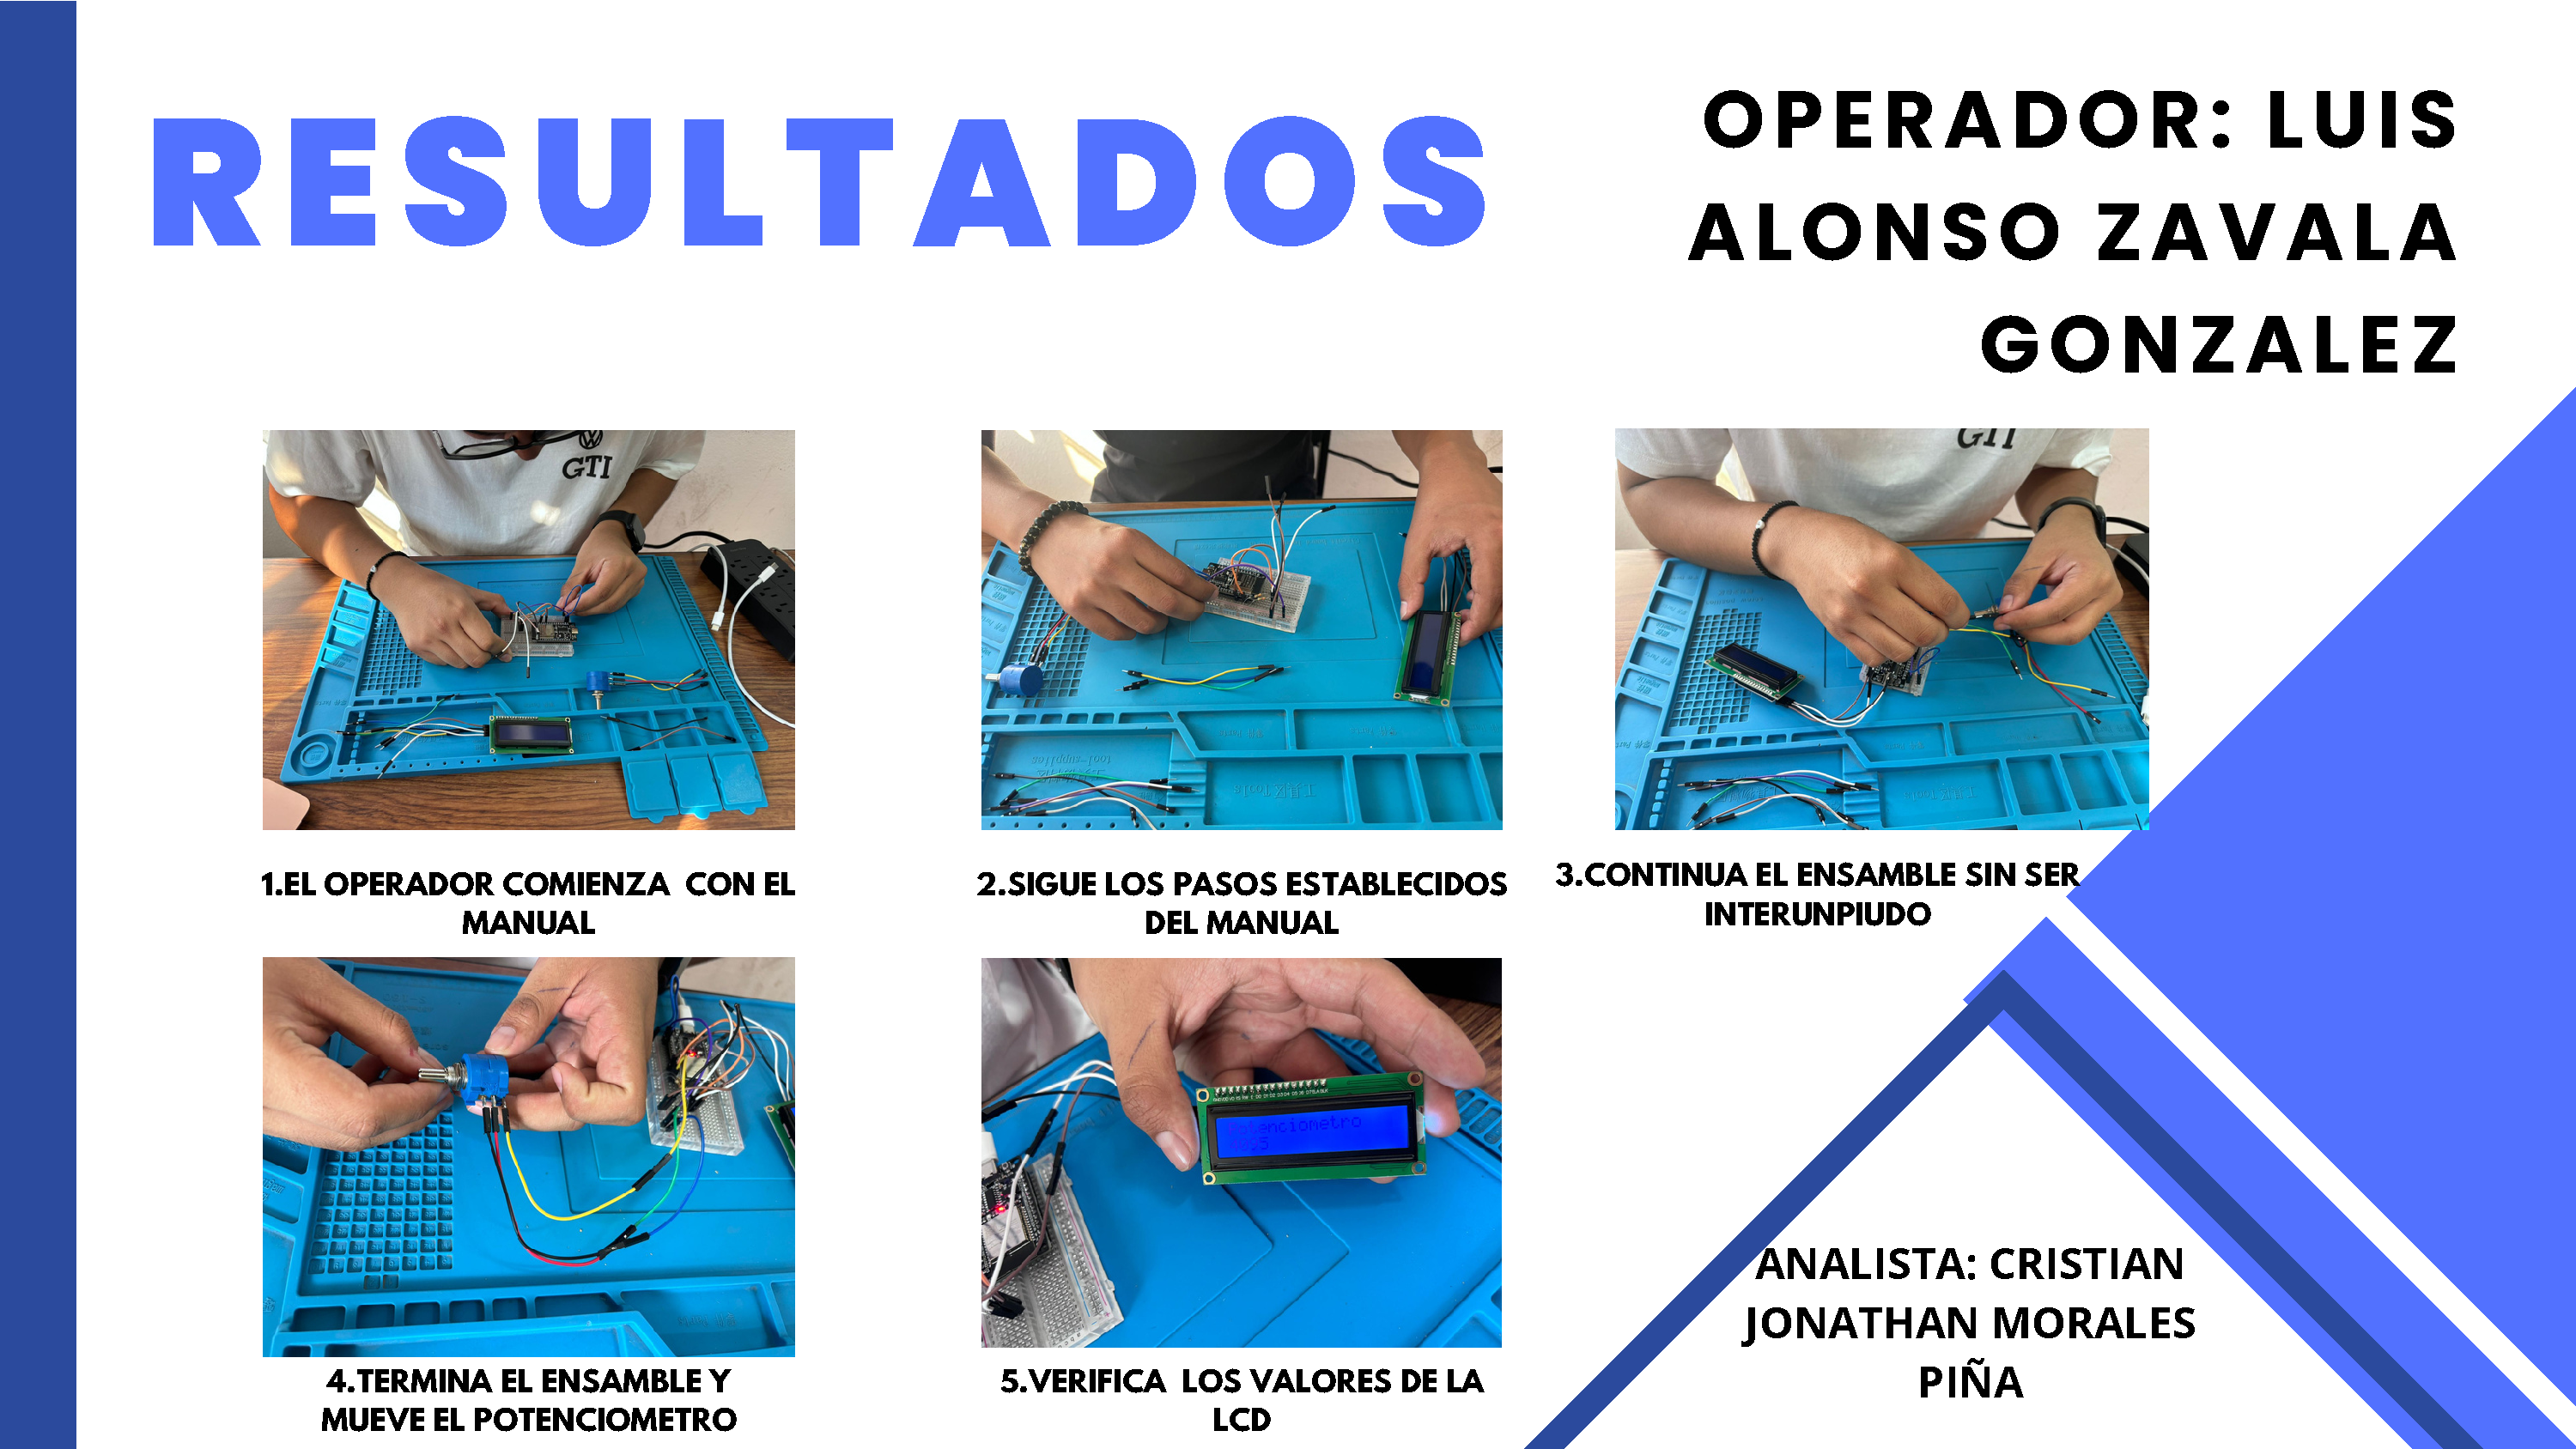
\includepdf[pages=-]{18/img/resultadosDeEnsamble.pdf}
     %%%%%%%%%%%%%%%%%%%%%%%%%%%%%%%%%%%%%%%%
     